% !TEX root = DesignDocument.tex


\chapter{Testing}
\label{ch:testing}

% This section describes the approach taken with regard to system and unit testing.    This chapter does not describe the outcome of those tests.    

\section{Overview}
\tab The testing approach is based on automated unit testing where available and manual testing with instructional testing steps recorded. Website testing, file conversion testing, mobile application testing, and component integration testing are all recorded and documented separately. The purpose of the product tests is to ensure that the features described in the user stories and project specification are met and work as intended. The manual tests for each user story are described below.

\section{Dependencies}
\tab The main testing framework for the Azure website is Microsoft's C\# testing framework. The file conversion needs no external testing framework as it is tested manually for accuracy. The database schema and implementation is provided by the Microsoft Entity Framework package, in which stable releases are guaranteed functional, however testing is done by verifying state persistence across publications.


 \section{Website}

 \subsection{Overview}
 \paragraph{}
 The website is a hosting service for uploading, downloading and managing the users files. Microsoft's ASP.NET MVC was used to create the website and Azure was used for its web hosting and file storage tools.
 
 \paragraph{}
 Users can create an account to store and share 3D models with other users. Once a user has an account, they can upload a 3D model as one of the websites supported file types. A user can download the model as any of the supported file types or generate a QR code that can be used for quick download using the mobile app or any other QR code readers.

\subsection{User Interface}
The user interface was designed to be very simple. The UI is comprised of four main pages with a navigation bar to get the pages
    \paragraph{Public Content Page}

        \begin{figure}[H]
        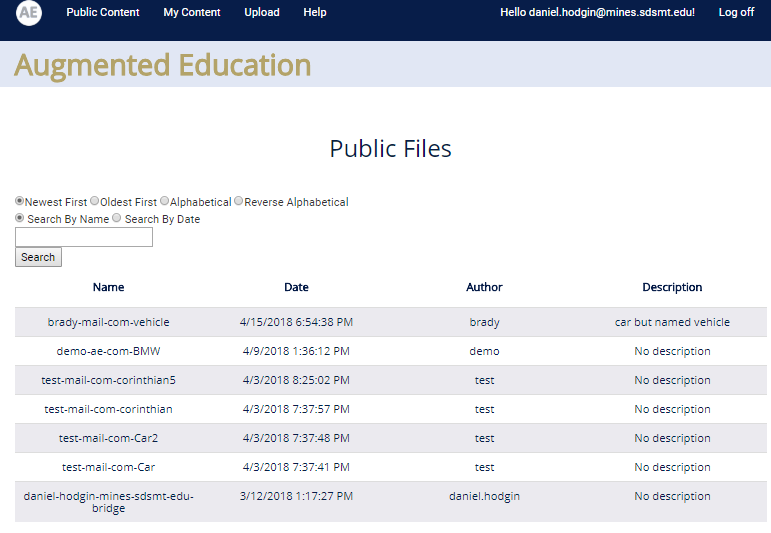
\includegraphics[width=0.5\textwidth]{Web/PublicPage}
        \centering
        \caption{Public Content Page}
        \label{fig:PublicContent}
        \end{figure}

        This is the main landing page for the website. From here users are able to browse the public files to download and generate QR code. Users do not need to be signed in or have an account to access the information on this page.

    \paragraph{My Content Page}
        \begin{figure}[H]
        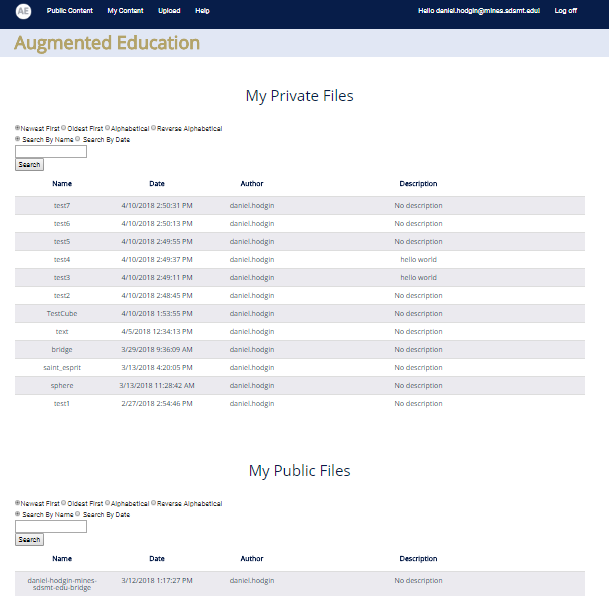
\includegraphics[width=0.5\textwidth]{Web/MyContent}
        \centering
        \caption{My Content Page}
        \label{fig:MyContent}
        \end{figure}

        This page will display all of the content that a user has uploaded. Here a user can browse their private and public files to download and generate QR codes. Users also have the ability to delete files. Users must have an account to access this page.

    \paragraph{Upload Page}
        \begin{figure}[H]
        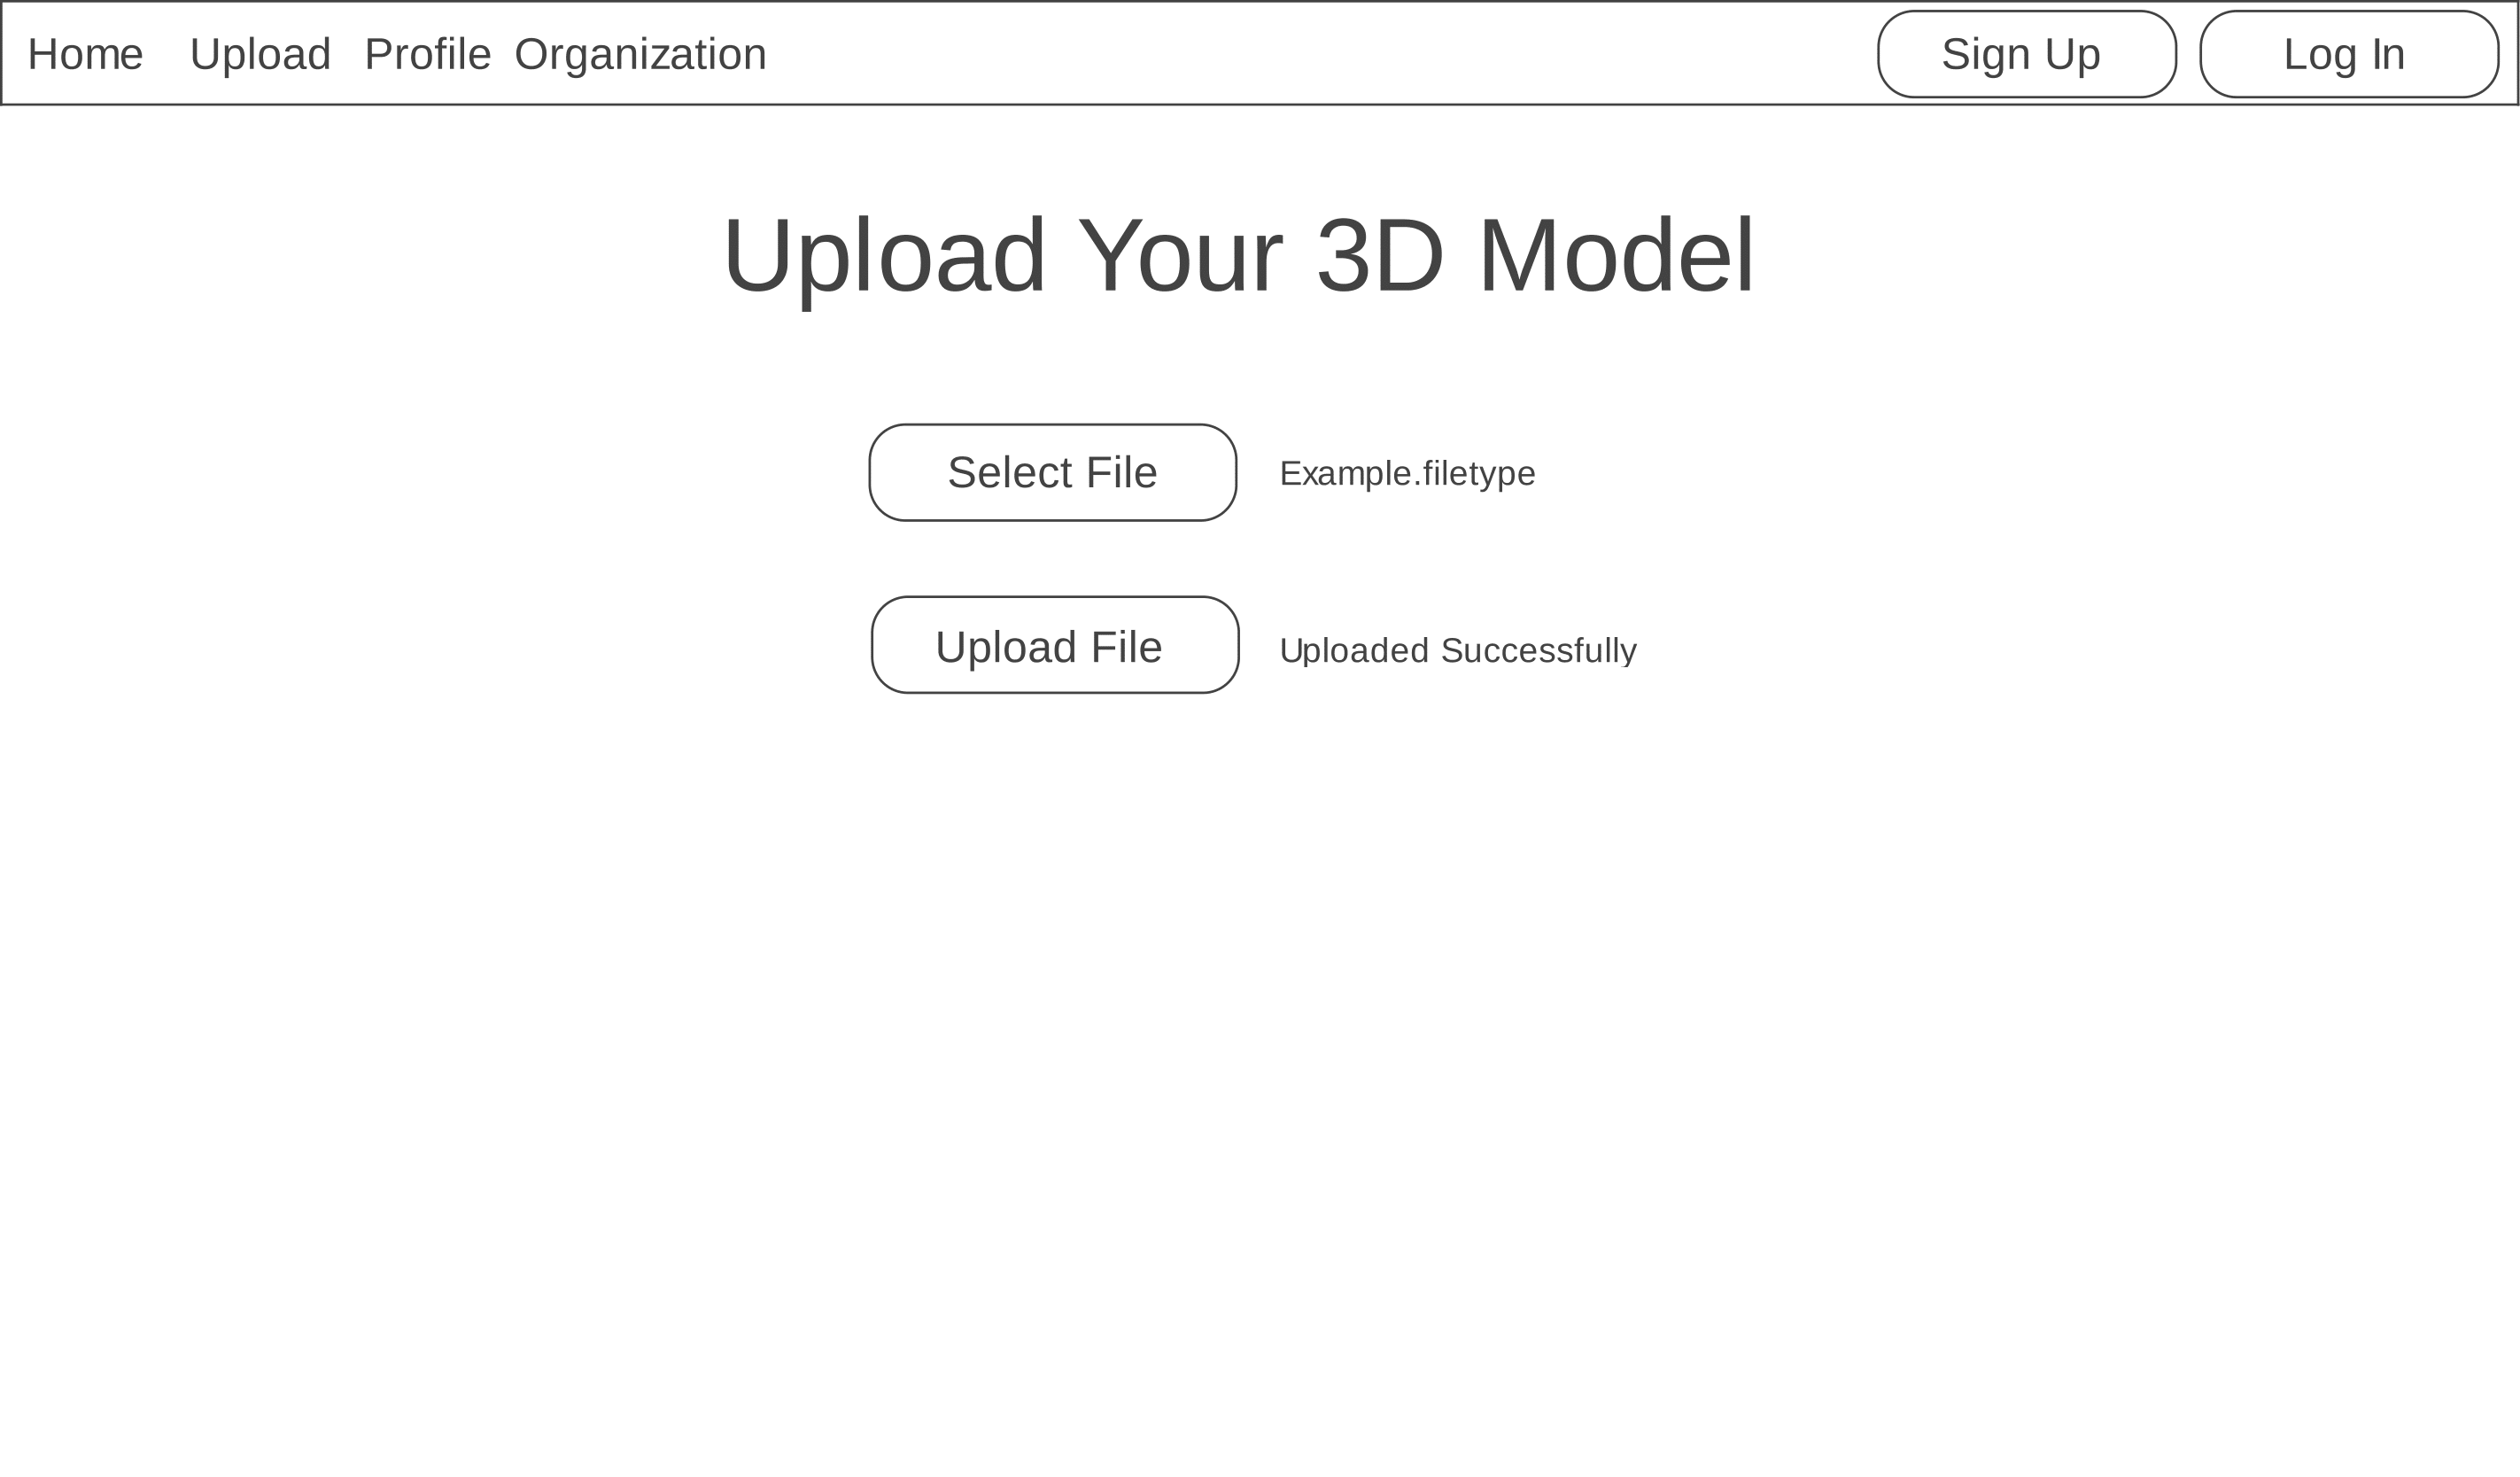
\includegraphics[width=0.5\textwidth]{Web/Upload}
        \centering
        \caption{Upload Page}
        \label{fig:UploadPage}
        \end{figure}

        This page will allow users to upload 3D models. Users can upload a material file if it is an OBJ file. The user can add a description, specify an alternate name, and make the file public. Users must have an account and be signed in to access this page.

    \paragraph{Help Page}
        \begin{figure}[H]
        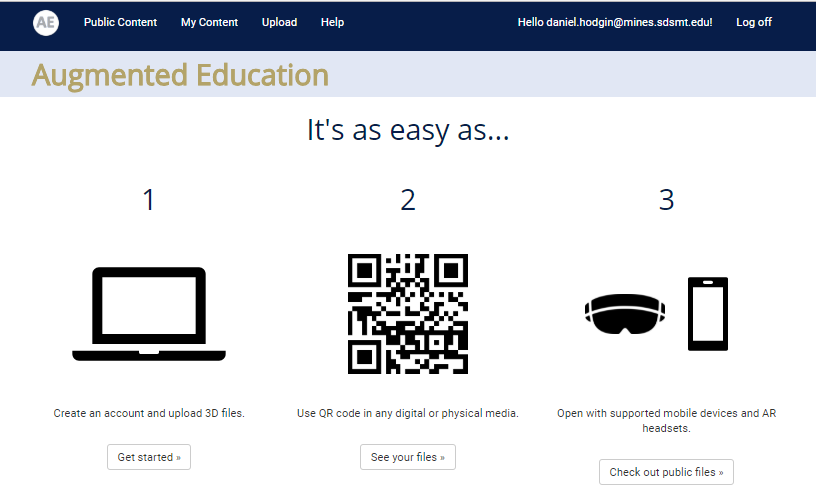
\includegraphics[width=0.5\textwidth]{Web/Help}
        \centering
        \caption{Upload Page}
        \label{fig:HelpPage}
        \end{figure}
    
        This page just gives a simple tutorial on how to uses the website.

\subsection{Technologies Used}

    As stated earlier in this document, this product is making use
    of the Microsoft environment for its tools. Below is an in-depth 
    breakdown of the tools currently being used:

    \begin{itemize}
    \item ASP.NET MVC
    \begin{itemize}
        \item An MVC web architecture, where the backend logic is written in controller classes
        that send and receive data from the client.
        \item It allows for dynamic html pages using a Razor syntax. Razor allows
        you to embed C\# Code into the html and execute logic.
    \end{itemize}
    
    \item Azure
        \begin{itemize}
            \item Microsoft cloud hosting services.
            \item Allows for simple database and web hosting.
            \item Paid features are offered free to students.
        \end{itemize}
    \end{itemize}

    These tools make up the core development of this website. The website is also
    making use of other smaller packages to handles user authentication and database management.

    The website also implements the file conversion software that is described later.
    The file conversion was written in C++, so it couldn't be compiled with the website.
    The workaround was that the file conversion was compiled into an executable that can be used through a system command to convert the file.


    \subsection{Data Flow}
    The website acts as an intermediary between the user and the cloud. Data flow for the website can be broken into a upload and download data flow.

    \paragraph{Upload Data Flow}
    \begin{itemize}
        \item Once a user upload a file it is temporarily save on the server.
        \item If the file is not a FBX file it is converted to a FBX file.
        \item The file is then uploaded to Azure blob storage for long term storage.
        \item The file on the server is then deleted on a sucessful upload to Azure.
    \end{itemize}

    \paragraph{Download Data Flow}
    \begin{itemize}
        \item When a user requests to download a file or generate a QR code, the file name and type is sent to the server.
        \item The server pulls the file from Azure and temporarily save it to the server.
        \item If a download is requested, it does a conversion if nessessary and send the file to the user.
        \item If a QR code is generated, it does a conversion if nessessary and then saves it back to Azure storage and returns a link to the file in Azure embedded in a QR code.
        \item 
    \end{itemize}


\subsection{Design Details}

    \subsubsection{Overview}

    The website was written in C\# with the ASP.NET MVC framework. The main logic
    of the website are contained in two controllers
    \begin{itemize}
        \item Upload Controller
        \begin{itemize}
            \item Handles upload from client to the server.
            \item Uses File Conversion executable to convert to .fbx
            \item Stores file on the web.
        \end{itemize}
        \item Download
        \begin{itemize}
            \item Uploads Model tag from client to server.
            \item Finds associated store model.
            \item Returns model to the client.
        \end{itemize}
    \end{itemize}

    \subsubsection{Code Structure}
    As stated before the website is using ASP.NET MVC framework. 
    The logic happens in the controllers and is split up into the upload and download controller.
    
    \paragraph{Parameter Passing}
    \hfill \break
    The main functions that are being used are the upload and download function.
    
    \begin{itemize}
        \item Upload Function
        \begin{itemize}
           \item HttpPostedFileBase - http message sent from client to server containing the file
           \item The message is parsed to retrieve the file and save to the web.
        \end{itemize}

        \item Download Function
        \begin{itemize}
            \item input string ModelTag - string containing the reference tag to the model.
            \item output httpresponse - http message sent from server to client containing the file. 
        \end{itemize}
    \end{itemize}

% !TEX root = DesignDocument.tex

\section{File Conversion Testing}
    The file conversion was manually tested using a variety of inputs to ensure robust and consistent performance. As there are two libraries (assimp and FBX SDK), they were both manually tested for simple functionality as they were implemented. Manual tests included sending through file types that could be inputs for assimp and making sure that the files made it to the FBX section and output the correct file format (FBX). Some of the input file types tested included common and expect file types such such as STL, OBJ, DAE etc. Unsupported file types were also tested and appropriate errors from the conversion libraries were received. The file types supported by the system are available in Table \ref{tab:suportedfiletypes}. Large files were also tested to gauge how long the system could take to process files of different sizes. There are certain limitations on the HoloLens hardware regarding file size and complexity. Users are properly notified of these limitations by the HoloLens platform should they be an issue. The HoloLens limitations are not formerly noted here as they are already anticipated to change with future updates.  

    Files with embedded textures were also tested to ensure textures get converted with the file. With the file types tested, such as OBJ and FBX, the textures converted with the files as expected. The HoloLens default 3D file viewer does not currently support colors or textures, thus these features have not yet been able to be tested.

    Test files of varying complexity were gathered from a variety of sources to ensure maximum coverage by the Augmented Education platform. The following files comprised the original test group used to ensure proper conversion to a FBX format and rendering on the Microsoft HoloLens:
    \begin{itemize}
        \item An OBJ sphere generated in Maple.
        \item An FBX column provided by Dr. Brent Deschamp of SD Mines.
        \item An OBJ sine wave generated in Maple.
    \end{itemize} 
    
    A number of files of varying format type from \url{http://free3d.com} were also tested. These sample files included a car, building, spaceship, Batman, and other unique files. 
    
    Cheldon was also able to receive large sample architectural files in FBX format from a relative. One architectural file rendered in the HoloLens, but the other two were too large to be supported by the device's current limitation for meshes and vertices able to be rendered in the viewer.

    Conversion examples can be seen in Figures \ref{Car-FBX}, \ref{Car-OBJ}, and \ref{Car-STL}.  
    
    In Figure \ref{Car-FBX}, a 3D model for a car in FBX format was acquired. This file was used to test conversion to OBJ format, the result of which can be seen in Figure \ref{Car-OBJ}. Figure \ref{Car-STL} is an STL file generated from the FBX file, using a DAE file as an intermediate format between the FBX SDK and assimp libraries. The STL file does not contain the colors or smooth surfaces that are present in the other file types, which is a limitation of the STL file format. This system works for converting STL $\rightarrow$ FBX as well, but the colors would not be present in the final file because that information is not contained in the STL. 
    
\begin{figure}[H]
    \centering
    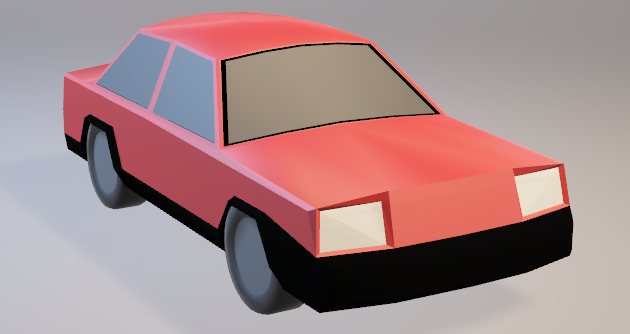
\includegraphics[width=\textwidth]{Car-FBX.png}
    \caption{Car FBX File}
    \label{Car-FBX}
\end{figure}

\begin{figure}[H]
    \centering
    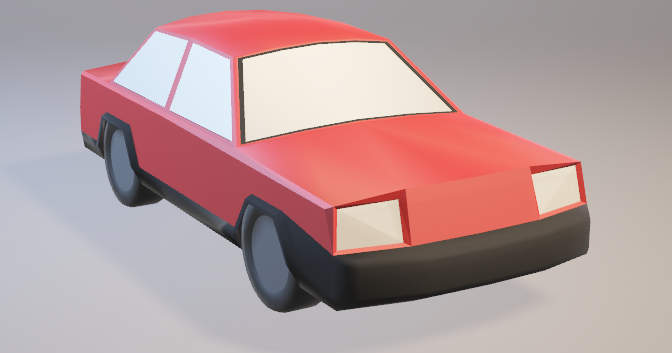
\includegraphics[width=\textwidth]{Car-OBJ.png}
    \caption{Car OBJ File}
    \label{Car-OBJ}
\end{figure}

\begin{figure}[H]
    \centering
    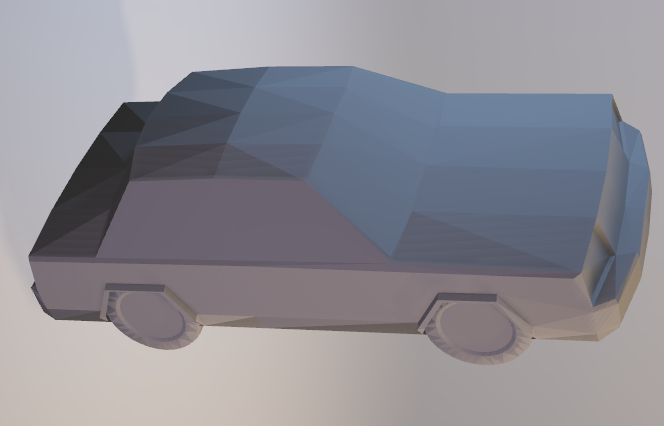
\includegraphics[width=\textwidth]{Car-STL.png}
    \caption{Car STL File}
    \label{Car-STL}
\end{figure}



\section{Mobile Testing}
    Testing for the mobile app was primarily done manually. This is because most testing was done on visualizing files and verifying the app performed as expected.  It was also verifying that HTTP packets were as expected going to and from the phone.

    When error messages are printed to the user of the app, a toast is displayed.  A toast is the small box that pops up on the lower section of the screen.

    \subsection{Files}
        A variety of files were used throughout development to test functionality of the app. Some sample files were found on \url{https://free3d.com}. Some files were provided from Dr. Deschamp and others were generated in Maple. Different files were used to test that colors were working both in the MTL and as PNGs. Additionally, large and small files were tested to see how the app reacted to more complex files. The BMW file seen below is an example of a complex file that doesn't render well in the app and demonstrates the limitations of the app.
        
        \subsubsection{Colors}
        
            A major feature requested for the app was to be able to display colors. The example below shows a simple sphere with a proof of concept that colors do work. The car is a more in-depth example that shows multiple colors on the same model.
            
            \begin{figure}[H]
                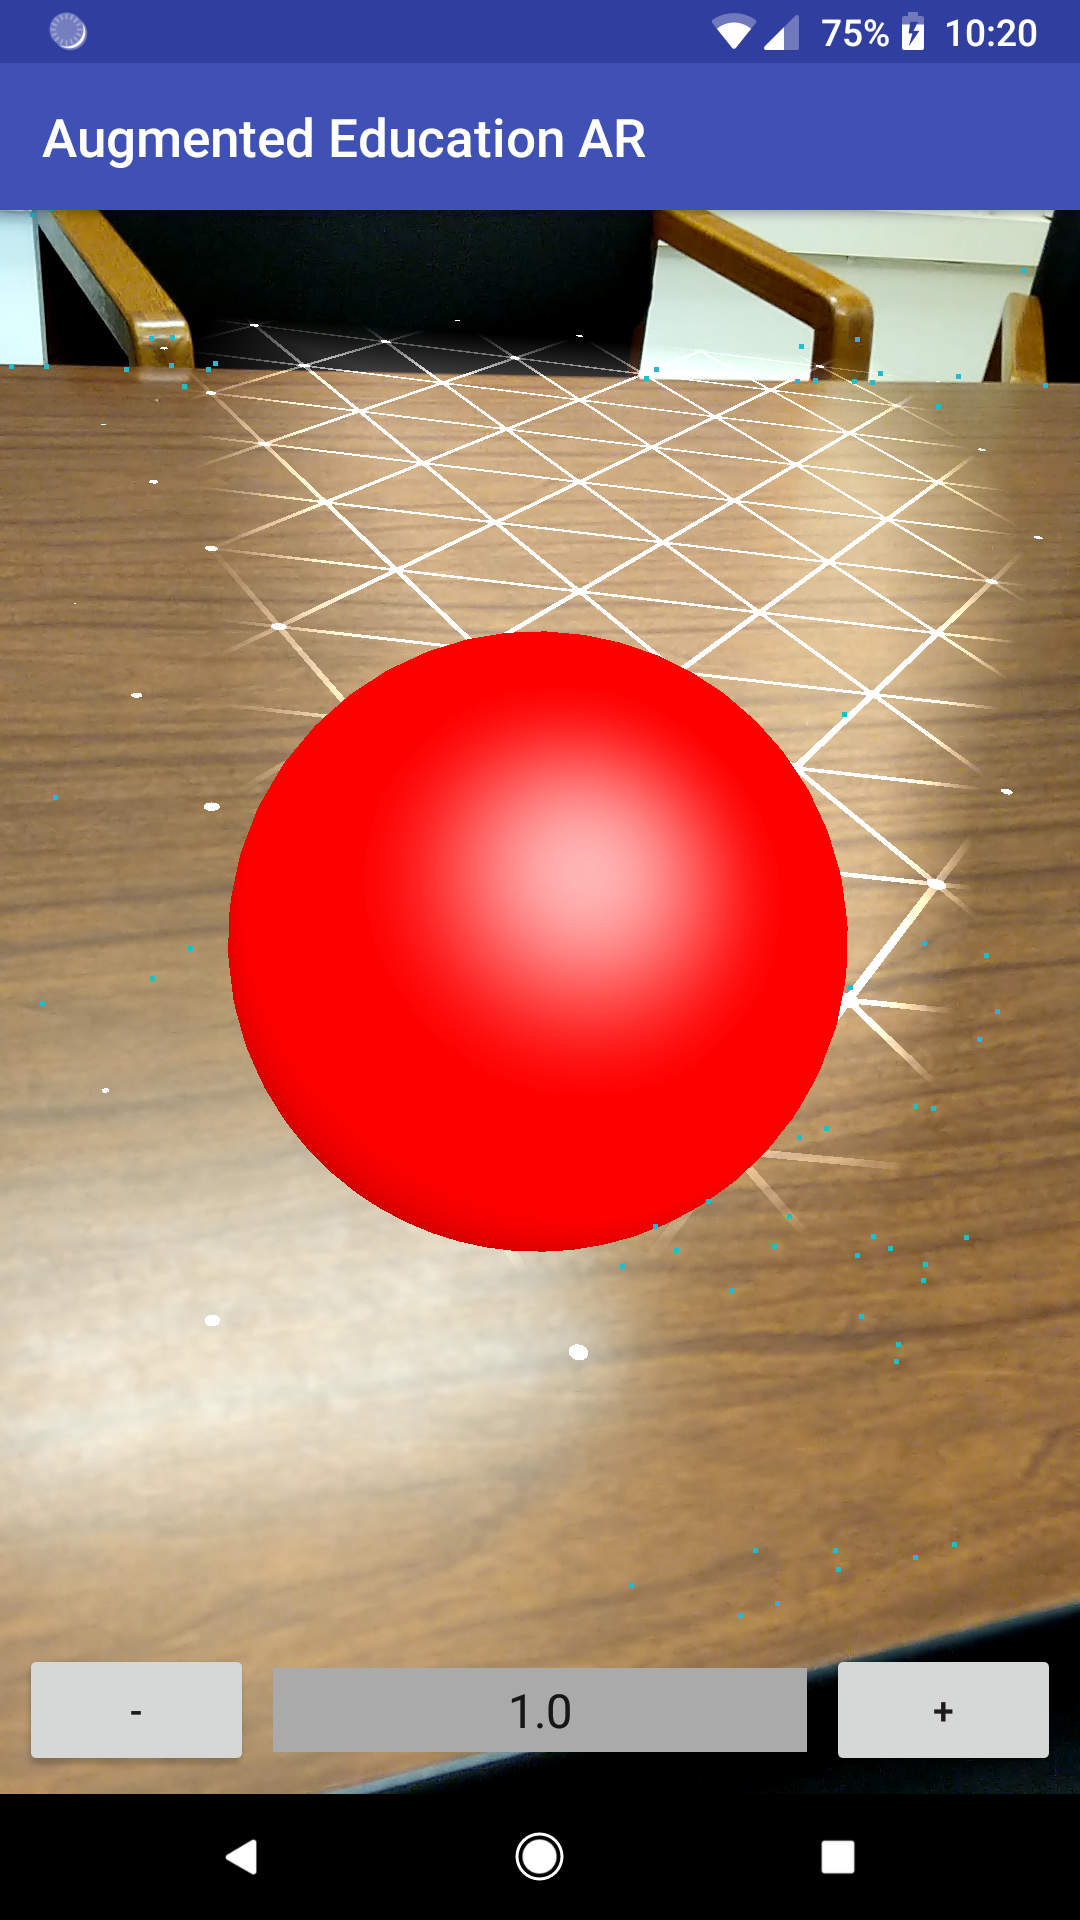
\includegraphics[width=0.5\textwidth]{Mobile/Mobile_RedSphere}
                \centering
                \caption{Colors - Red Sphere}
                \label{fig:mobileRedSphere}
            \end{figure}

            \begin{figure}[H]
                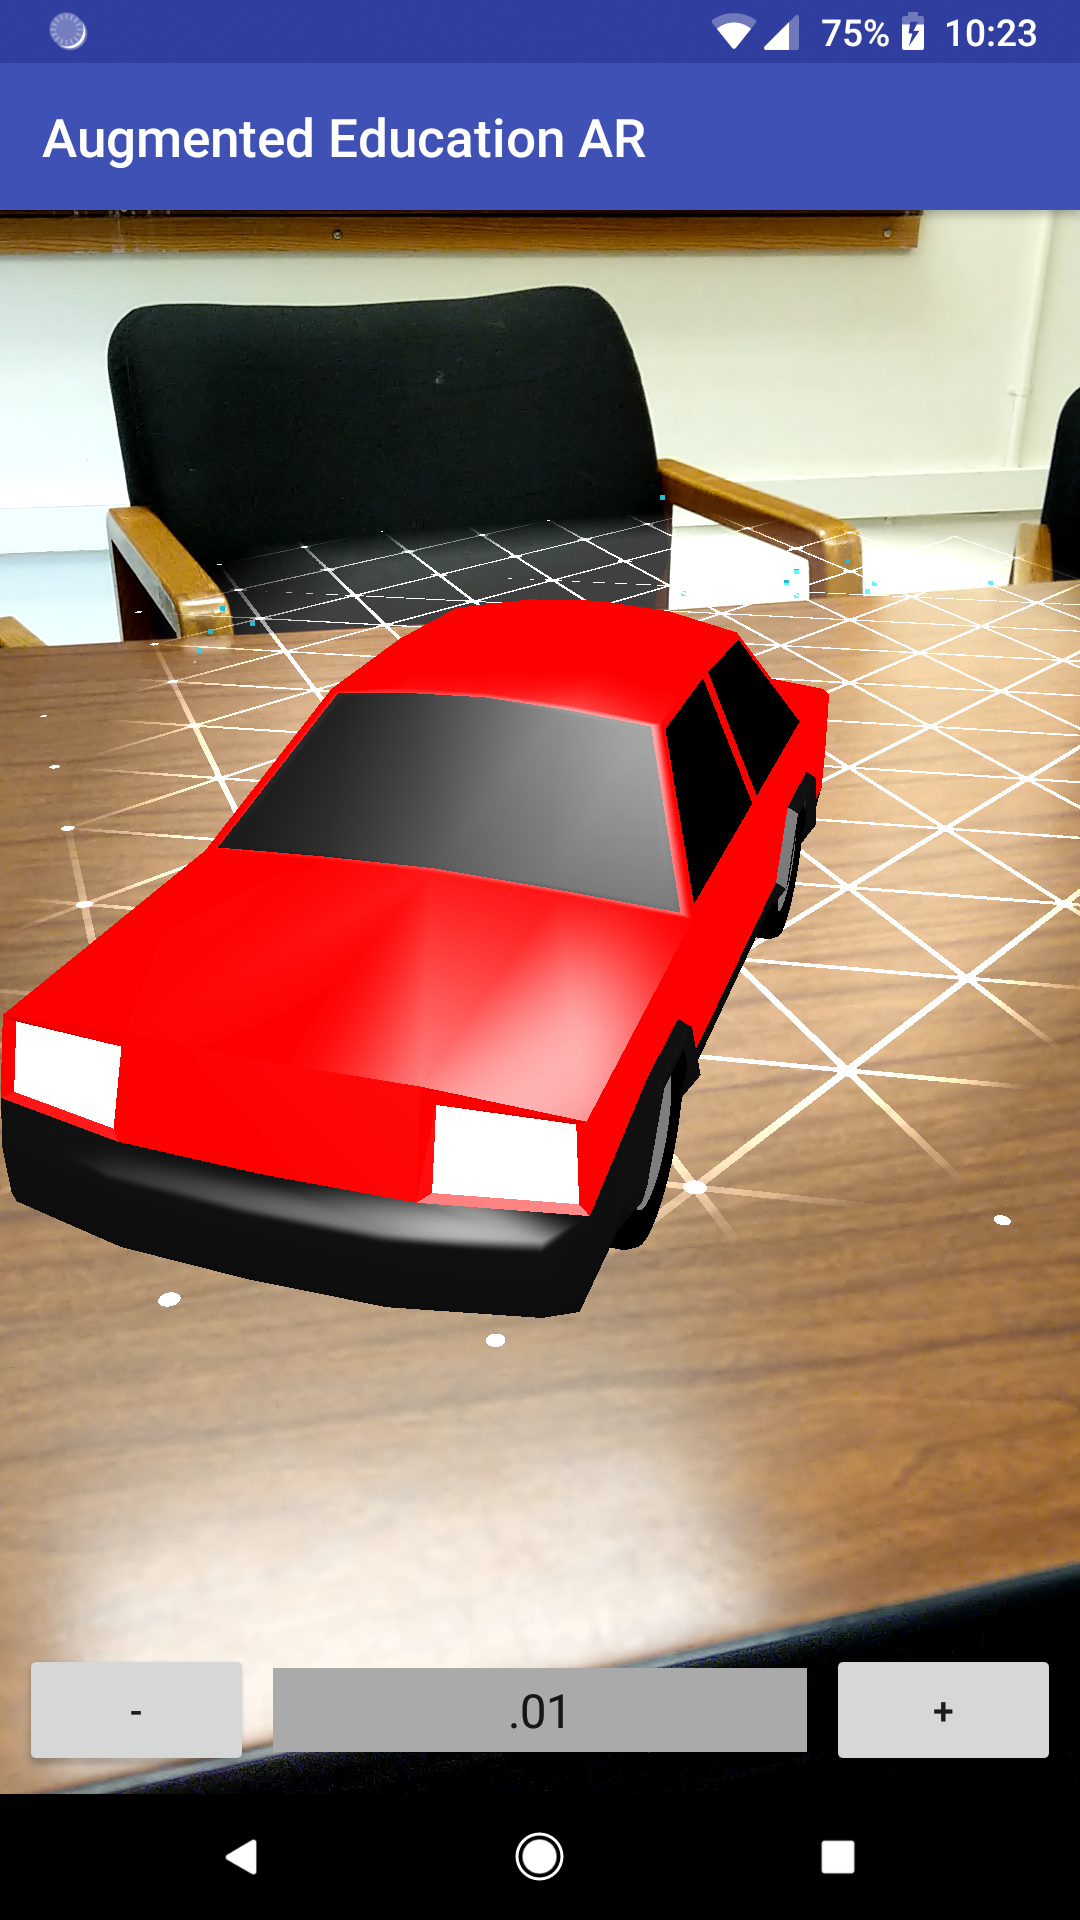
\includegraphics[width=0.5\textwidth]{Mobile/Mobile_Car}
                \centering
                \caption{Colors - Car}
                \label{fig:mobileCar}
            \end{figure}
        
        \subsubsection{Large Files}
        
            One main concern was that 3D files can get large and complex. The BMW is an example of this because it has 51,318 vertices while the sphere only has 2,258. It took a longer amount of time ($\sim$5 seconds) to load this file and it draws poorly, showing a limitation of keeping track of so many vertices.
            \begin{figure}[H]
                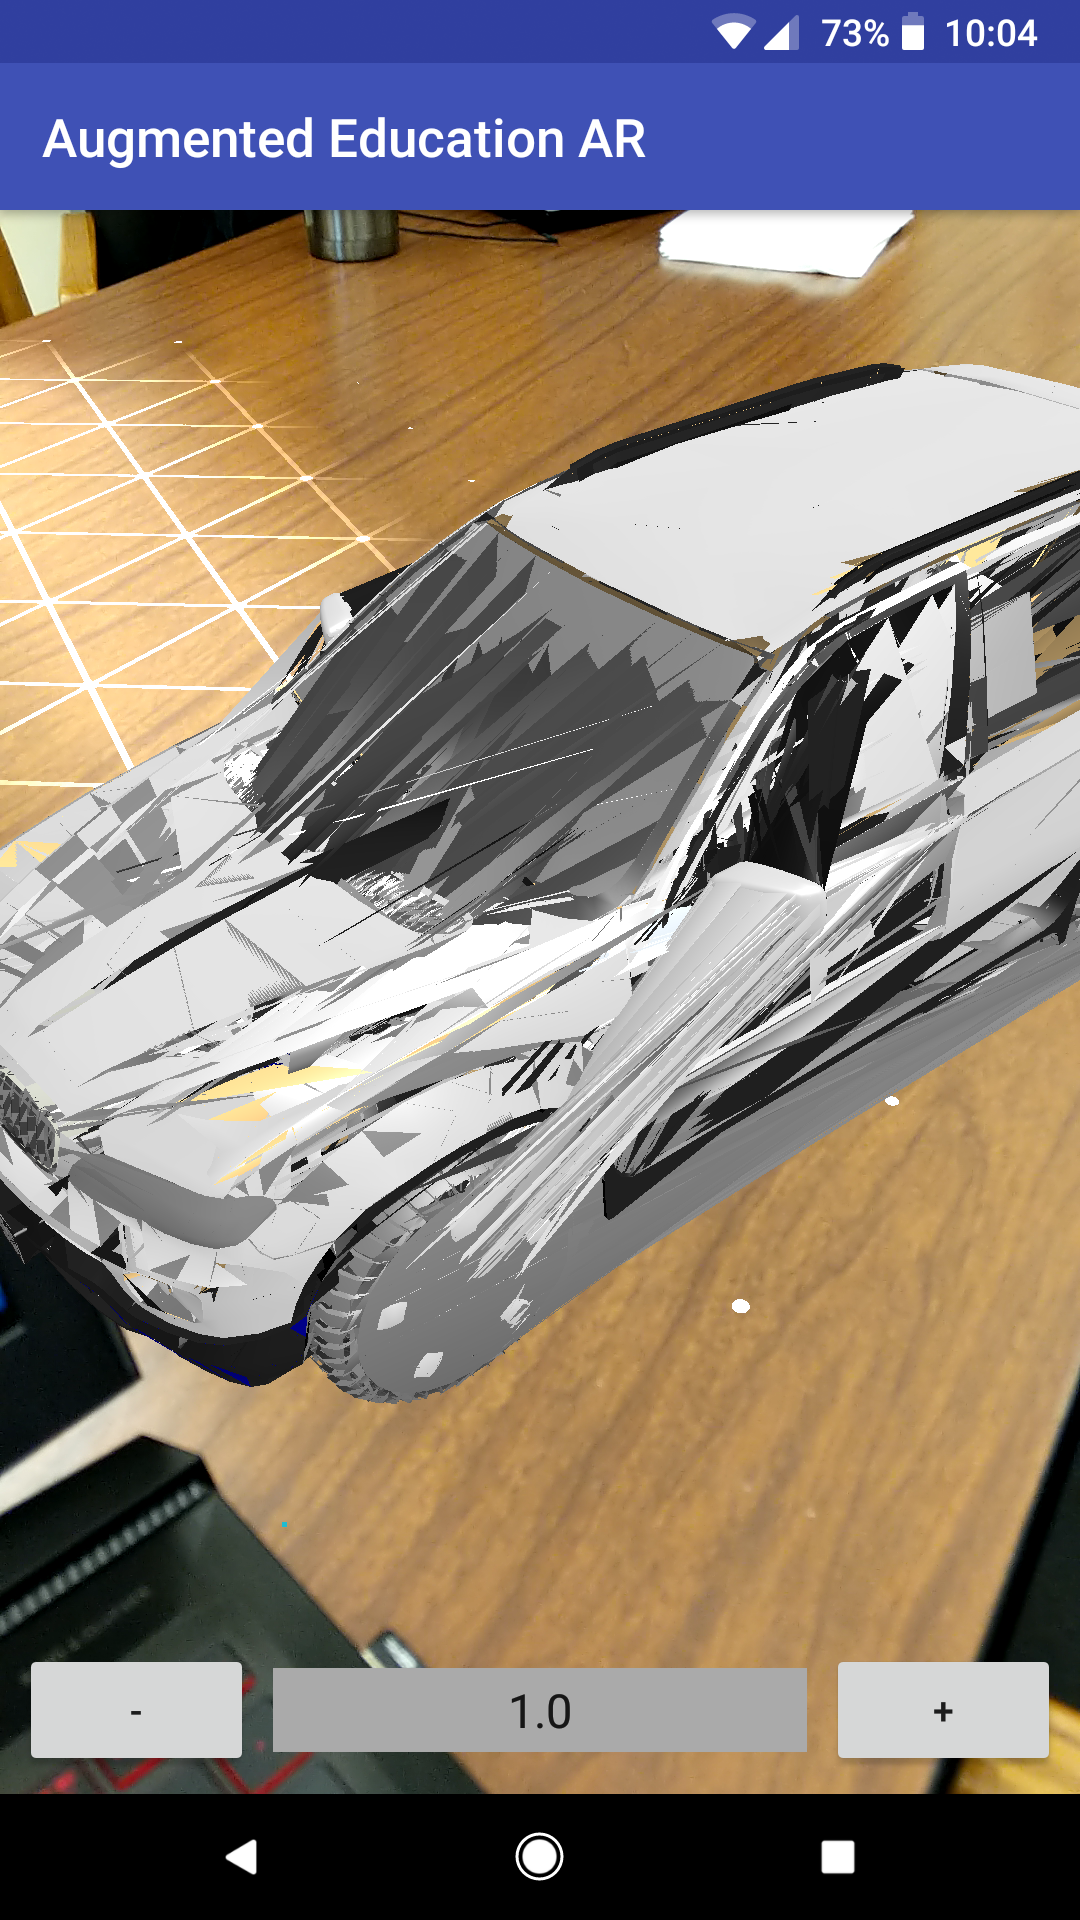
\includegraphics[width=0.5\textwidth]{Mobile/Mobile_BMW}
                \centering
                \caption{Large File - BMW}
                \label{fig:mobileBMW}
            \end{figure}
    
        \subsubsection{Small Files}
            A simple test used especially at the beginning of development to test that models would draw. The sphere is a typical example of something generated from Maple. 
        
            \begin{figure}[H]
                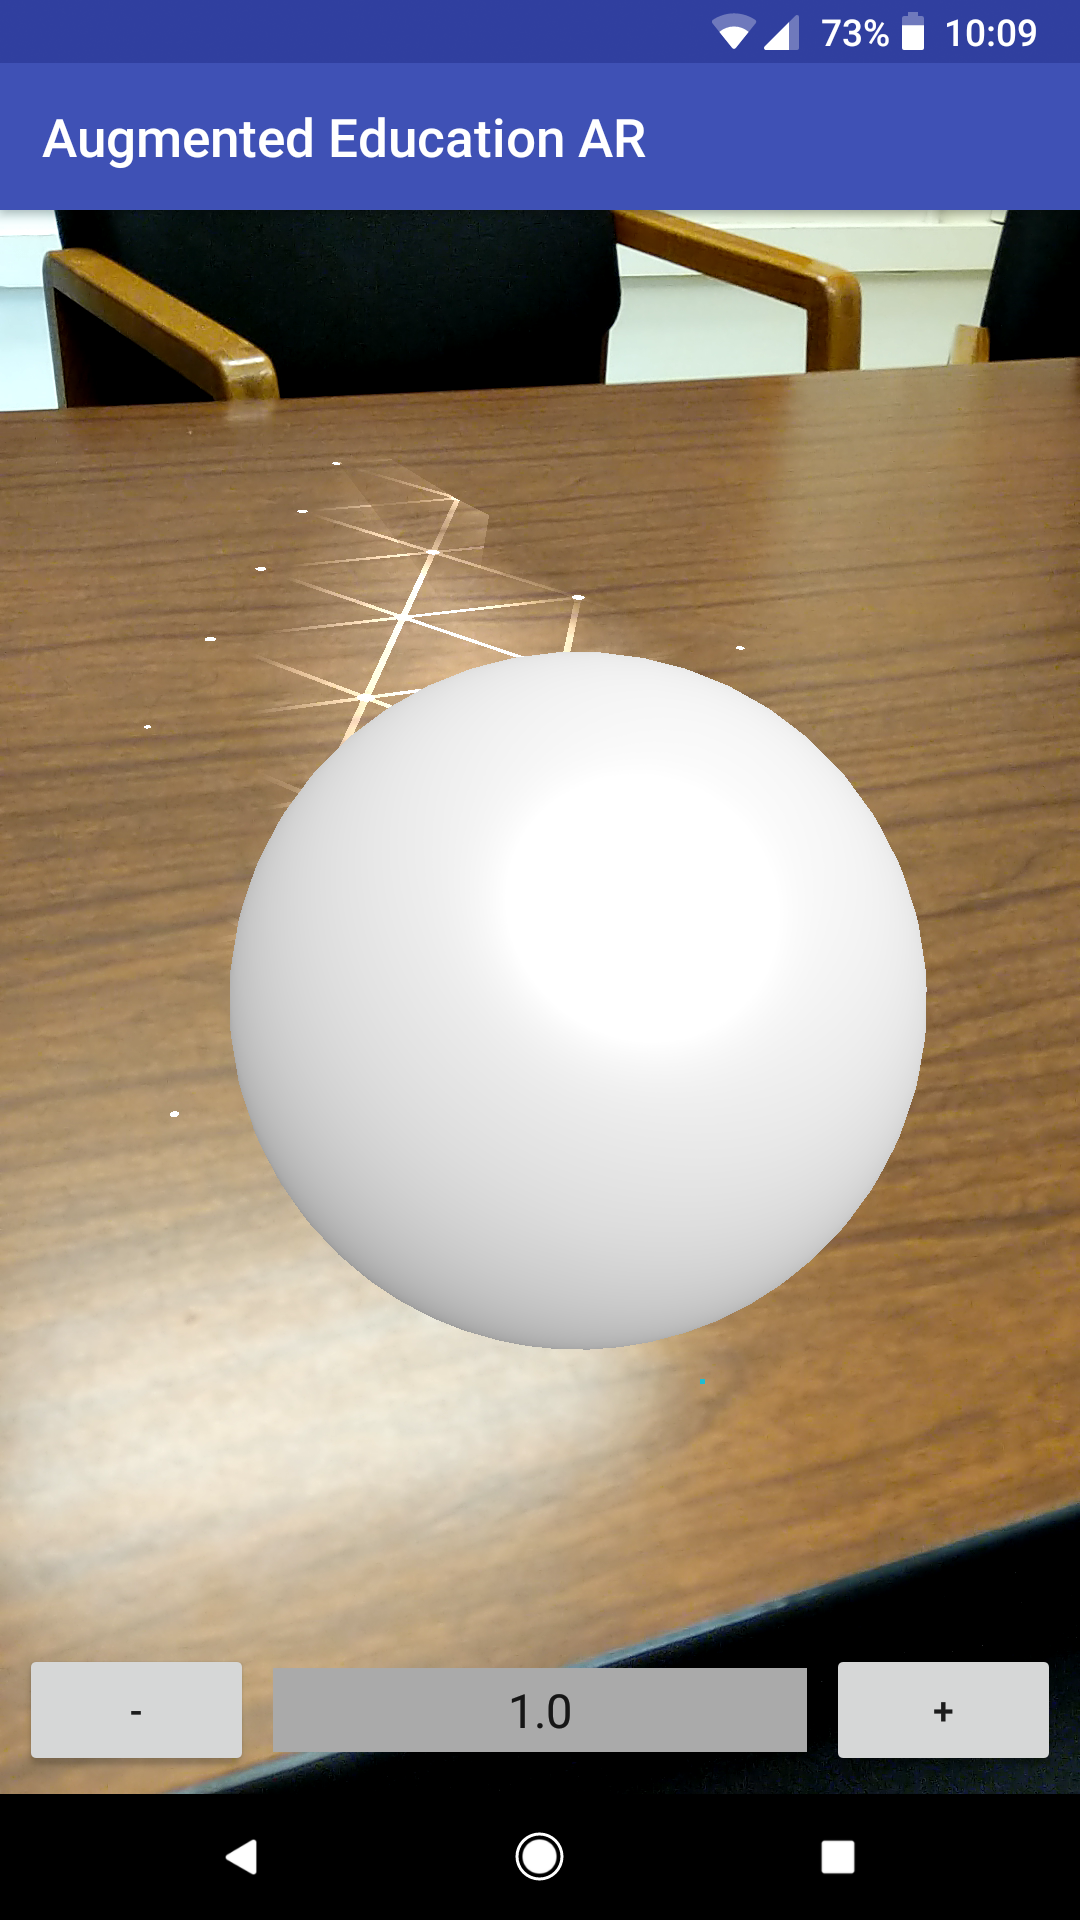
\includegraphics[width=0.5\textwidth]{Mobile/Mobile_Sphere}
                \centering
                \caption{Small File - Sphere}
                \label{fig:mobileSphere}
            \end{figure}
            
        \subsubsection{Embedded Images}
            
            Some 3D modeling software generates OBJ files with PNG textures referenced in the MTL instead of defining RGB values. It was necessary to test that these files were also supported by the app after adding extra functionality for them. Figure \ref{fig:mobileEmbeddedPhone} shows the PNG texture working, but it doesn't match the intended plot perfectly (Figure \ref{fig:mobileEmbeddedWindows}). This is because the app currently does not support drawing multiple images on top of each other yet.
        
            \begin{figure}[H]
                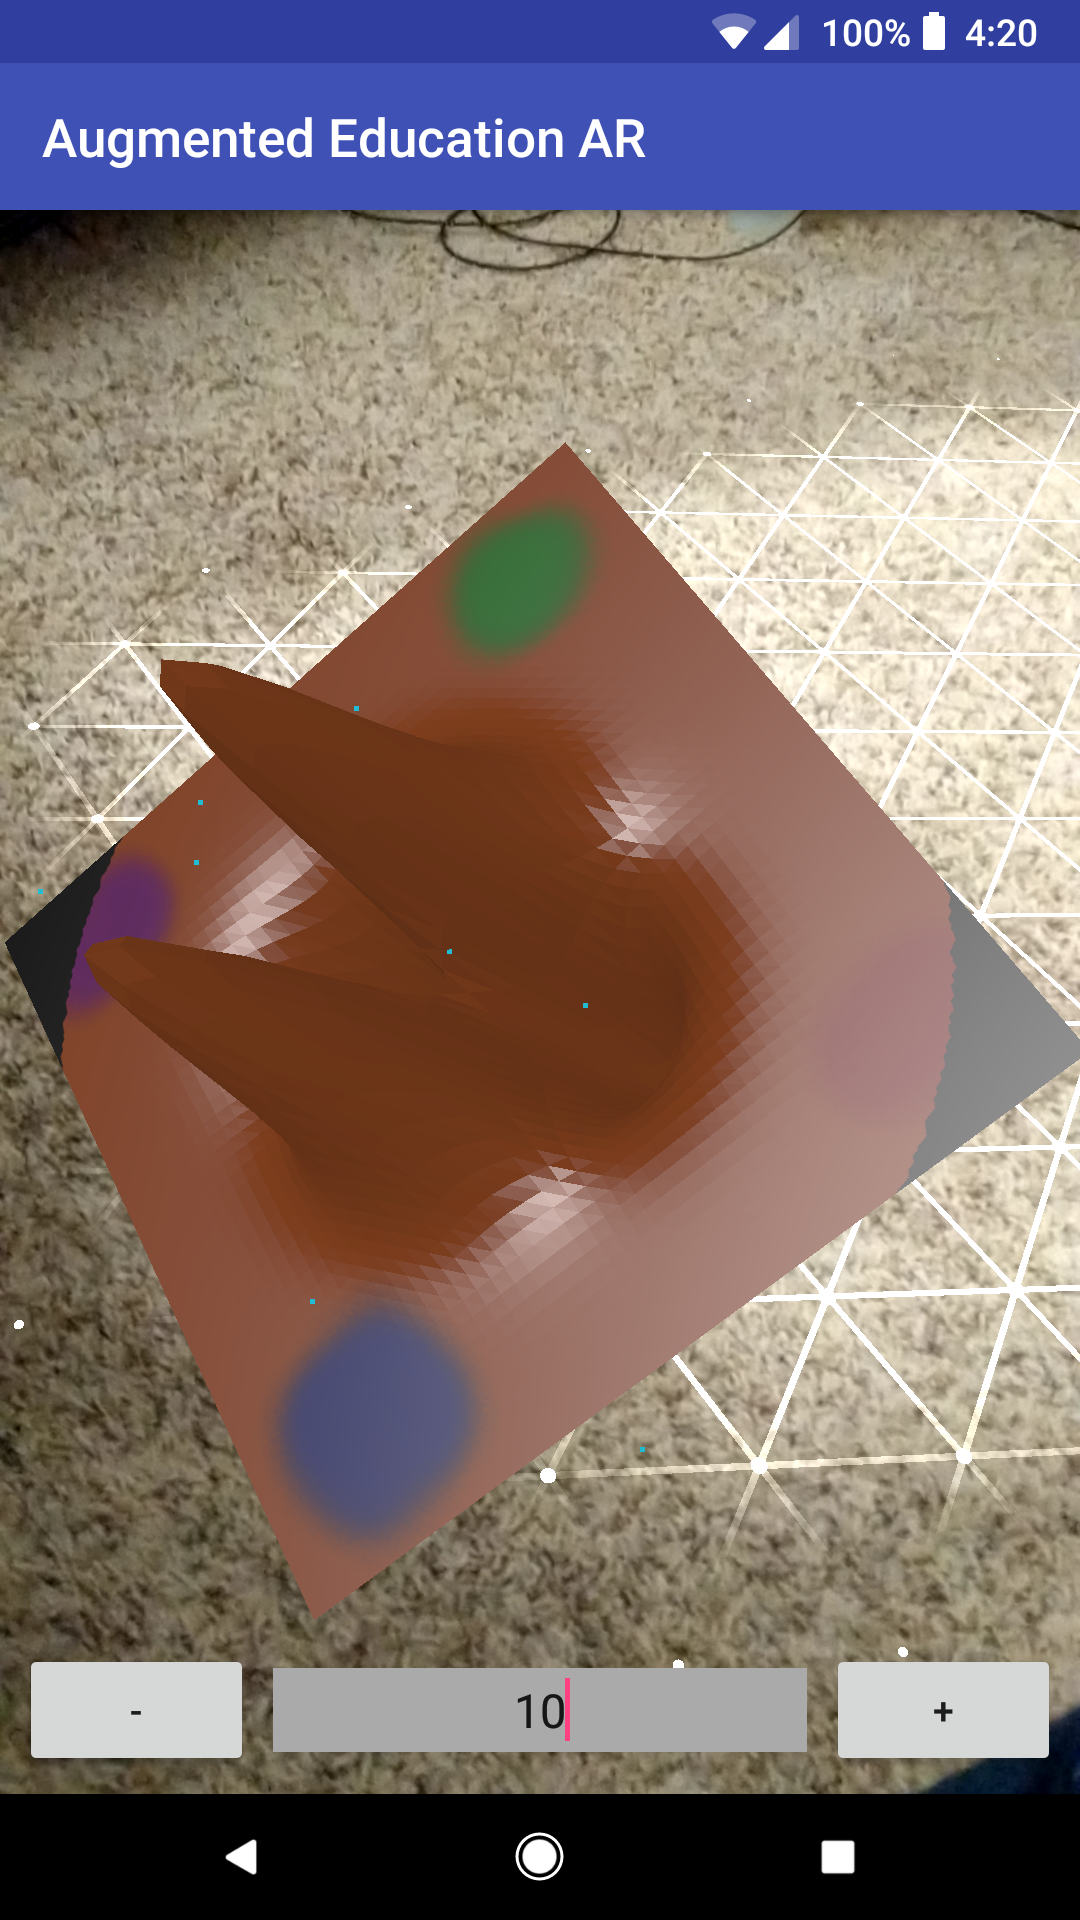
\includegraphics[width=0.5\textwidth]{Mobile/Mobile_ImagesPhone}
                \centering
                \caption{Embedded Image - Viewing on the phone}
                \label{fig:mobileEmbeddedPhone}
            \end{figure}

            \begin{figure}[H]
                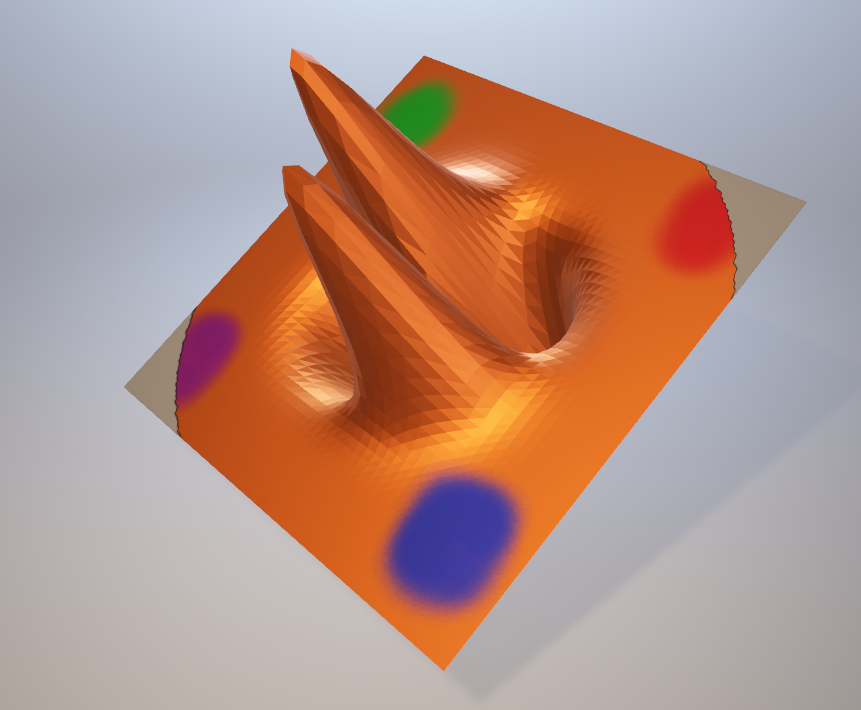
\includegraphics[width=0.5\textwidth]{Mobile/Mobile_ImagesWin}
                \centering
                \caption{Embedded Image - Viewing in the Windows Viewer}
                \label{fig:mobileEmbeddedWindows}
            \end{figure}

        \subsubsection{Scaling}

            Different models scale differently when initially drawn in the app. A scale factor of 1.0 on one model may be too small or too large, making the model difficult to visualize. To remedy this, the app provides an option to increase or decrease the scale factor, as well as change the step so models of different scales can be adjusted properly. Maple models generally need a larger scale factor (approx 3.0) while others like the car need to be adjusted by 0.1 at a time.
        
    \subsection{Web Interface}

        Another major component of the mobile app was the communication with the website.  If the app can display the models, there is little purpose if there is no method to get the models onto the phone.  The web API provided by the web team provides a method for communicating with the website.  It is done using the Volley library, provided by Google.  It abstracts the low level sending/receiving of networking communication away from the developer.  The code for these interfaces in primarily located in the \texttt{WebAccessor} Java class.

        Testing has shown that while the website is on Azure, the responsiveness is not always the best.  It is not infrequent to receive timeout errors on requests.  When this occurs, a message is displayed to the user.
        
        \subsubsection{Endpoints}\label{sec:Mobile_Auth}
        
            The endpoints used by the mobile application allow the app to: authenticate with the website, get a list of owned models, and download a model.  The endpoints were tested using Postman (to make sure the response was what was expected), the Android Studio debugger to make sure the correct fields were set, and a packet capture application to view the actual HTTP message sent from the phone.

            \paragraph{Authenticate}

                The authentication endpoint allowed the user to provide a username and password to get access to the website.  If the user entered valid credentials, an auth token is returned that allows the application to make requests on behalf of the user.  The auth token is used in the other API calls to the server.

                This API call is only performed on the Main Activity screen (the login page).  If a user is not authenticated, the user cannot continue through the app unless they select the Offline Mode button to not perform future web communication tasks.  A success of this component was, if the user supplied valid credentials, a valid auth token was returned.  Otherwise, an error message should be printed.  The testing was performed manually by trying invalid usernames/passwords.  In these cases, the website did not provide a valid auth token.  When correct usernames/passwords were entered, an auth token is returned.

                The Postman view that was used to test the endpoint (on the web side) is shown in Figure \ref{fig:mobilePostmanGetAuthToken}.

                \begin{figure}[H]
                    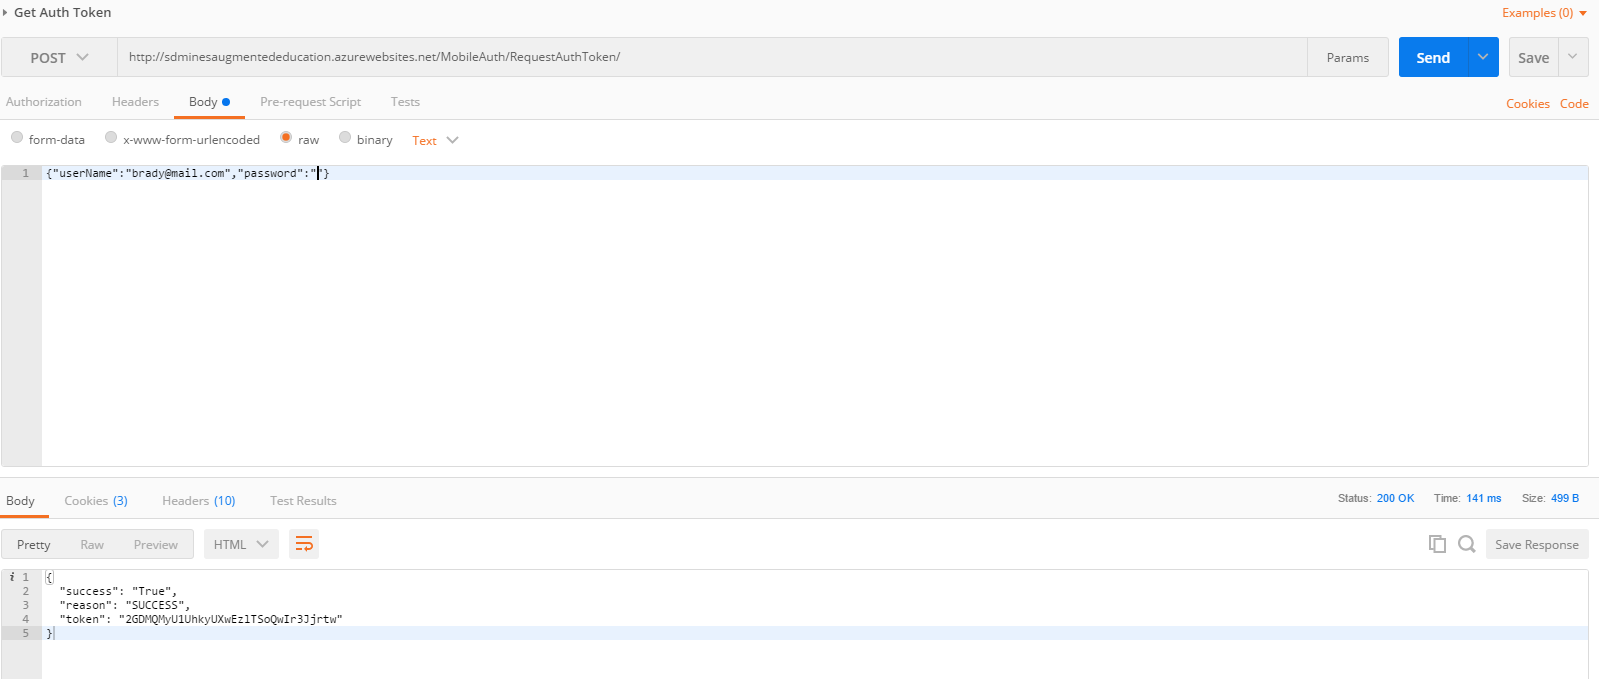
\includegraphics[width=0.75\textwidth]{postman_GetAuthToken}
                    \centering
                    \caption{Postman - Get authentication token}
                    \label{fig:mobilePostmanGetAuthToken}
                \end{figure}
                
            \paragraph{List Models}

                Another endpoint that is used by the mobile device is the one to get a listing of files owned by the user.  Like with the authentication token request, this call was tested manually to ensure the HTTP packets were well formed, and as expected.  Postman was again used to help test.  Figure \ref{fig:mobilePostmanListFiles} shows the Postman setup to send a request for a file listing.  
                
                \begin{figure}[H]
                    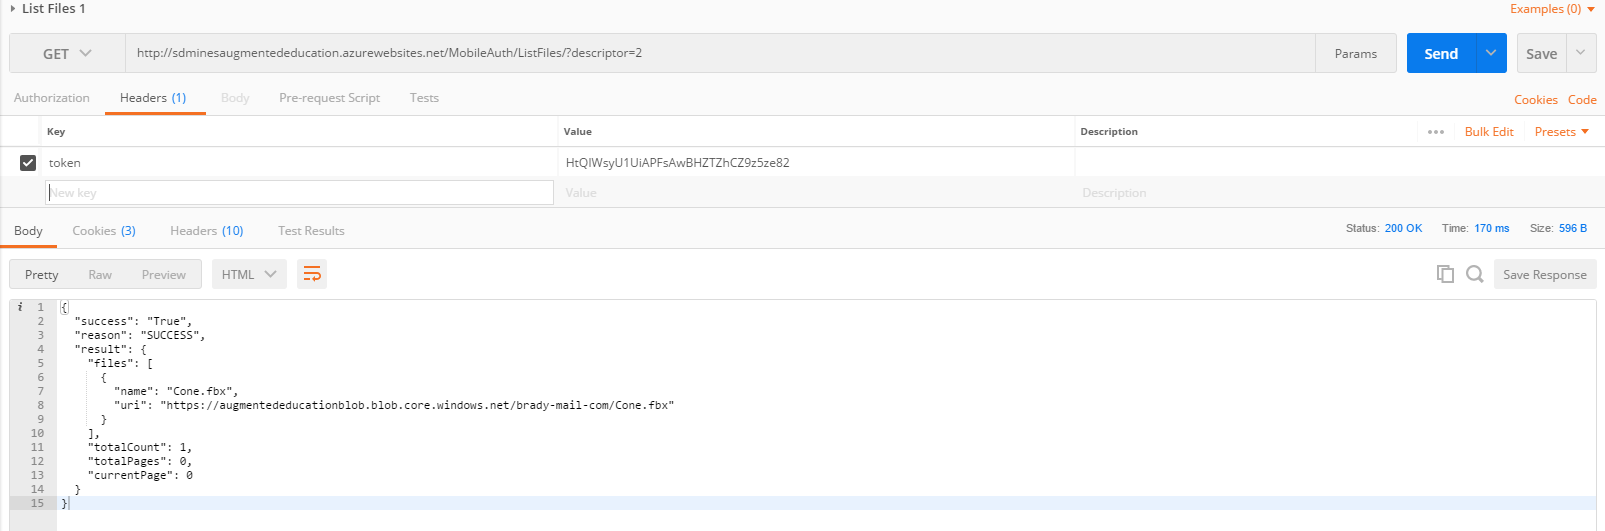
\includegraphics[width=0.75\textwidth]{postman_ListFiles}
                    \centering
                    \caption{Postman - List files}
                    \label{fig:mobilePostmanListFiles}
                \end{figure}
                
                Note, the \texttt{descriptor=} at the end of the URL, as it is used to state which files are desired for download.  An agreement was made between the mobile and web teams on what the levels should be.  There is an enumeration defined in the Java code with more details on the values and meanings.  Testing the different values showed a bug in the web code that always caused an error on the mobile device.  This issue was fixed by the web team.
            
            \paragraph{Download Model}

                Downloading a model includes contacting two endpoints.  One is used to get a temporary link to actually download the file, and the next downloads the file from that URL.  This is used so the phone can store the long term location, and get a temporary active URL to get the file.  Testing for these sections again included using Postman, and using a web browser to facilitate the download.  The Postman settings to get the temporary URL are located in Figure \ref{fig:mobilePostmanDownloadFile}.

                \begin{figure}[H]
                    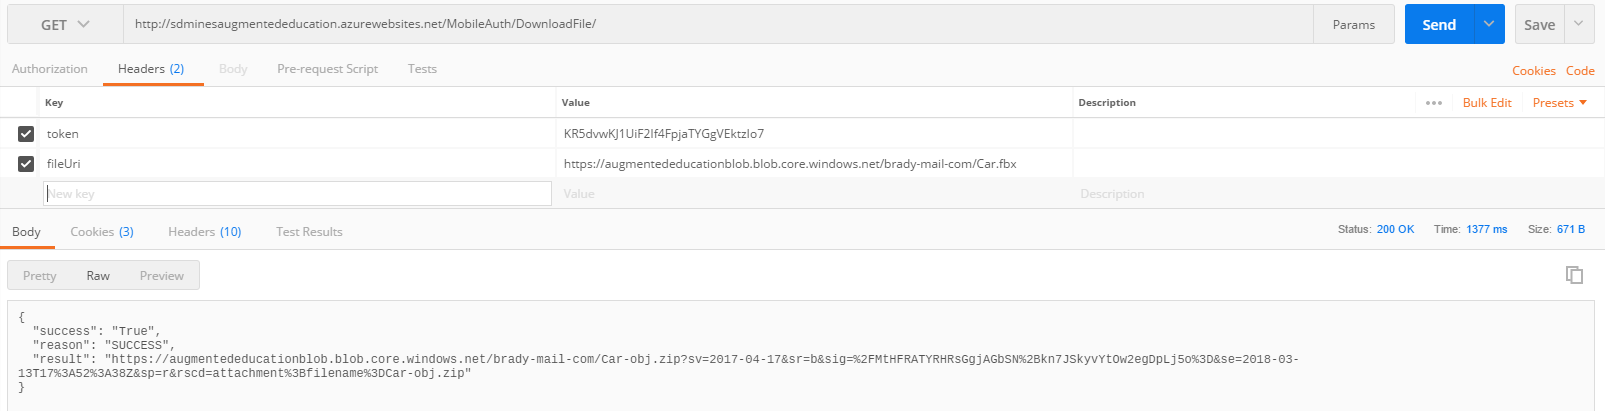
\includegraphics[width=0.75\textwidth]{postman_DownloadFile}
                    \centering
                    \caption{Postman - Download a file}
                    \label{fig:mobilePostmanDownloadFile}
                \end{figure}

                The field \texttt{result} contains the temporary URL.  It would then be put into a web browser (typically Firefox or Chrome) and the file is downloaded.  The file downloaded should be in the OBJ file format, since it is the one that is parse-able by the phone.  The website should use the file conversion software ensure this.  When the models are downloaded, they are stored in a \texttt{Models} directory on the phone.  The file system on the device can be viewed with the Downloads app.  Note, if the model is downloaded, and it does not show up in the file structure, the phone should be restarted.  Commonly, the files do not show up until the device is restarted.  A new folder will be created in the \texttt{Models} directory.  This is because one OBJ model can have multiple other models associated with it, including MTL (material) files and images.  When the models are downloaded, a zip archive is actually downloaded and extracted.

                Future developers should be aware of how the models are saved from the Android download manager.  When making the call for the download manager to do the download, a final path/file name must be provided.  This can cause issues if the file is saved with the wrong extension, especially if the files are viewed on the developers computer (and not just on the phone).
        
        \subsubsection{No Internet}

            Since internet can be less than reliable on cell phones, it was important to test if the there was no internet on the phone.  This was done by turning off Wifi on the testing phones (as they do not have cellular activated).  As expected, if there is no internet, an error message is displayed to the user that the communication was unsuccessful.
        
    \subsection{Offline Mode}
        
        When preparing for the Senior Design Fair, the mobile team decided that it would be a good idea to add an offline mode so the user can view models without having to authenticate with the server.  This was because the Wifi capabilities at the fair would be slim to none.  Therefore, an "Offline Mode" button was added to the login page to allow the user to continue offline.  Testing needed to be done on this to only show models registered as on the phone, as the user would not be able to download remote files without first authenticating.  This was tested and implemented in the application.  The application will not get a list of models from the website or download files from the website in offline mode.  The rest of the functionality (such as viewing the models) remained the same, which was as desired.

    \subsection{QR Code Scanning}
        
        To test that the app was scanning QR codes as expected during development, the team tried a number of different QR codes found online and printed on objects around. There were a surprising amount of these objects on hand with printed QR codes to test with. Testing on these gave an idea of the performance of the QR code scanner for varying QR code sizes.

        The scanner worked with QR codes that pointed to the 3D model downloads.  One difficulty of testing this was the way that the list of models was populated.  When the list was originally populated, all models owned by the user, and models that were public were added to the list.  So, all of the models that the user could access would already be in the list, so scanning a QR code would do nothing.  A later revision changed this so only privately owned files were added to the list, so QR codes can now usefully be scanned. Once the team had the functionality to embed the download link in a QR code, the team tested downloading a number of files manually using their respective QR codes.

    \subsection{Database}
        
        To test the database, the team primarily tested manually by using the test 3D model files. The database is populated by all the models private to the user's account. The team verified that when models are added to the user's account, the database is updated with a listing of the new models. The database also adds entries for scanned QR code files.

% !TEX root = DesignDocument.tex

\section{System Testing}
Testing the system involved manually using the software as a user would.
The test relied on being able to access the website, upload a file, and being able to download the converted version of it.
This was successfully tested through manual tests and these features were present in the MVP.

% !TEX root = DesignDocument.tex

\section{System Integration Testing}

	\subsection{File Conversion and Web}
		
		Manual integration tests were performed while integrating the file conversion software with the website. The integration test was relatively simple and only required the executable to be uploaded to Azure and called as it would regularly be with user requests. Website and file conversion software integration was determined to be complete after multiple successful tests of the complete upload $\rightarrow$ conversion $\rightarrow$ download process.

	\subsection{Mobile and Web}

		Integration between the mobile app and the website takes the form of some endpoints the website will respond to when contacted by the mobile app. The endpoints were developed by the web team; however, the mobile team was consulted for what functionality was required for the app. Members from each group conferred to develop the following endpoints: Authentication, List Models, and Download Models.  As stated in Section \ref{sec:Mobile_Auth}, Postman was used to manually test the endpoints.

		One endpoint that could be created in future developments is the ability to get printable name for a file.  Currently, displaying the name of the file, especially from QR codes, works.  However, the name is very ugly as there is no way to get an easily printable file name.  Scanning a QR code will currently use the URL for the file on the website as the file name in the list. An endpoint for this would allow the phone to better display the models on the mobile device and has been listed as a future development consideration in Ch. \ref{ch:TODO}. 

% !TEX root = DesignDocument.tex

\section{Risk Analysis}
There are two main risks associated with this project. These risks pertain to the functionality of the project itself and the security of its data. Minimizing and preventing these risks are vital to providing quality software and positive relationships with users.

The first risk is that the software may fail to convert or render a given input file. This could be caused by the file being too large, complex, or corrupt for the system to handle. 

In regard to file security, some of the files uploaded may contain sensitive or confidential data. The platform has been designed with the most current security precautions available, but cybersecurity is ever-changing. Security precautions included by the developers may become outdated or deprecated. Additional risk lies in trusting third-party hosting services as these services are frequent targets of cybersecurity threat. 

The project also relies on the Identity and Entity Framework for file access authorization. While this framework is well-respected in the professional development community, it should be noted that the development group is trusting the integrity of the authorization process to this third-party resource.


% !TEX root = DesignDocument.tex

\section{Risk Mitigation}
To mitigate these risks, we have multiple strategies implemented to prevent the issues from happening in the first place.

Addressing the first risk of failed conversion or rendering, we will ensure product quality through rapid iteration and testing of MVPs. 
We have a variety of test files of varying sizes and formats that we have run through our system to make sure we cover many of the common (and uncommon) use cases.
Additionally, we aim to stay informed on the documentation of the libraries and platforms we use in our software to make sure we understand the capabilities and limitations of the tools we are using.
Especially for the file conversion software, we have researched which file types can be run through the libraries and have implemented that functionality in our product and need to communicate to our users which file types are acceptable for our system. 

For the second risk of data security, we try our best to examine and remove any possible security holes in our data flow.
We will need to analyze the website code to limit file access only to properly-privileged users. 
We also plan to implement features such as https and end-to-end encryption to maintain data security on our connections.